\RequirePackage[no-math]{fontspec}
\special{dvipdfmx:config z 0}
\documentclass[twoside, fontset=fandol, punct=kaiming]{ctexbook}
\usepackage[svgnames]{xcolor}
\usepackage{graphicx}
\ctexset{
    chapter = { 
        name = {章,},
        beforeskip = 1em,
        format = \Large\bfseries$\triangleright~$,
    },
	section = {
	  name = {,},
	  number = \chinese{section},
	  format = \large\bfseries,
	 }
}
\def\setminus{\,\mathord{\mathchar"226E}\,}
\usepackage[b5paper]{geometry}
\usepackage[scr=boondox]{mathalpha}
\usepackage{amsmath,amsfonts,amssymb,amsthm,euscript,fontspec,tocloft,fancyhdr,mathtools,enumitem,pgfplots,tikz-cd,xeCJKfntef}
\usepackage{tikz}
\usetikzlibrary{calc}
\usepackage{fixdif}
\usepackage[
    colorlinks,
    linkcolor = DarkTurquoise!60!black,
    anchorcolor = OrangeRed,
    filecolor = OrangeRed,
    urlcolor = OrangeRed,
    citecolor = Teal,
    linktocpage,
    hyperfootnotes = true,
    breaklinks = true,
]{hyperref}

\setlist[enumerate]{itemsep = 0pt, label=\roman*.}
\setlist[itemize]{itemsep = 0pt}
\setmainfont{lmroman10-regular.otf}[
    BoldFont = lmromandemi10-regular.otf,
    ItalicFont = lmroman10-italic.otf,
    SizeFeatures = {
        {Size = {-9}, Font = lmroman8-regular.otf},
        {Size = {9-14}, Font = lmroman10-regular.otf},
        {Size = {14-}, Font = lmroman17-regular.otf}
    } 
]
\setCJKmainfont{FandolSong-Regular.otf}[
    BoldFont = FandolSong-Bold.otf,
    ItalicFont = FandolKai-Regular.otf,
    SizeFeatures={
        {Size={-9}, FakeStretch = 1.05, ItalicFont = FandolKai-Regular.otf},
        {Size={9-}, FakeStretch = 1, ItalicFont = FandolKai-Regular.otf}
    } 
]

\renewcommand\implies{\DOTSB \,\Longrightarrow \,}
\DeclareMathOperator{\dom}{dom}
\newcommand\dif{\mathrel{\triangle}}
\renewcommand{\sectionmark}[1]{\markright {\uppercase{#1}}}
\fancypagestyle{fancy}
{    
    \fancyhead[OR]{\fontspec{lmsansquot8-oblique.otf}[FakeStretch=.85]\itshape\small\rightmark\qquad{\fontspec{lmsans10-boldoblique.otf}\thepage}}
    \fancyhead[LE]{\fontspec{lmsansquot8-oblique.otf}[FakeStretch=.85]\itshape\small{\fontspec{lmsans10-boldoblique.otf}\thepage}\qquad\leftmark}
    \fancyhead[LO,RE]{}
    \fancyfoot[C]{}
    \renewcommand{\headrulewidth}{0pt}
}
\pagestyle{fancy}
\let \mathcal \EuScript
\newlength \circlenumbertemp
\newlength \squarenumbertemp
\newcommand {\circlenumber} [1] {%
    \ifnum #1 > 9
        \circlenumbertemp = 0.18cm
    \else
        \circlenumbertemp = 0.12cm
    \fi
    \hbox{\begin{tikzpicture}[baseline = -.8ex]
        \draw [line width = .3pt] (0,0) circle (0.12);
        \node at(0,0){\makebox[0pt]{\resizebox{\circlenumbertemp}{!}{\textbf{#1}}}};
    \end{tikzpicture}}
}
\newcommand {\squarenumber} [1] {%
    \ifnum #1 > 9
        \squarenumbertemp = 0.18cm
    \else
        \squarenumbertemp = 0.12cm
    \fi
    \hbox{\begin{tikzpicture}[baseline = -.7ex]
        \draw [line width = .3pt, rounded corners = 1pt] (-0.12,-0.12) rectangle (0.12,0.12);
        \node at(0,0){\makebox[0pt]{\resizebox{\squarenumbertemp}{!}{\textbf{#1}}}};
    \end{tikzpicture}}
}
\renewenvironment{quote}{\begin{flushright}\small\kaishu\begin{minipage}{15em}\hspace*{2em}}{\end{minipage}\end{flushright}\medskip}
\makeatletter
\newcommand\fonttemp{\f@size}
\renewcommand\@makefnmark{\@textsuperscript{\scalebox{.8}{\circlenumber{\@thefnmark}}}}
\renewcommand\@makefntext[1]{%
  \hspace*{-2em}%
  \parindent 2em%
  \noindent
  \hb@xt@ 2em{\hss
  \normalfont
  \scalebox{1}[.9]{\circlenumber{\@thefnmark}}~}%
  #1}
\newtheoremstyle{innocent}{}{}
{\rmfamily\kaishu}{}
{\sffamily\bfseries}{}
{ }{\thmname{#1}\thmnumber{ #2}\,\mdseries\rmfamily\thmnote{$\left(\,\mbox{#3}\,\right) $}.~}
\theoremstyle{innocent}
\newtheorem*{theorem}{定理}
\begin{document}

\definecolor{titlegreendark}{HTML}{C1C998}
\begin{titlepage}
    \tikzset{help lines/.style=thick}
    \begin{tikzpicture}[overlay, remember picture]
        \filldraw[fill = titlegreendark!50!white, line width = 0pt, titlegreendark!50!white] (current page.south west) rectangle +(\paperwidth,\paperheight);
        \def\rectanglepath#1{\filldraw[fill = titlegreendark, line width = 0pt, titlegreendark, rotate = 45] #1 rectangle +(3,3);}
        \foreach\i in {-36,-30,...,18}{\foreach\j in {-36,-30,...,18}{\rectanglepath{(\i,\j)}\rectanglepath{(\i+3,\j+3)}}}
        \draw[help lines, step=.3cm, opacity = .02] (-30,-30) grid (30,30);
    \end{tikzpicture}
    \begin{tikzpicture}[overlay, remember picture, opacity = .1]
        \foreach \x in {1,...,500}{
                \pgfmathrandominteger{\a}{-1000}{500}
                \pgfmathrandominteger{\b}{-1000}{500}
                \pgfpathcircle{\pgfpoint{+\a pt}{+\b pt}}{+3pt}
                \color{titlegreendark!70!black}
                \pgfusepath{fill}
            }
        \end{tikzpicture}
    \begin{tikzpicture}[overlay, remember picture]
        \node[opacity = .2] at ([xshift = .5\paperwidth, yshift = -.5\paperheight]current page.north west){
            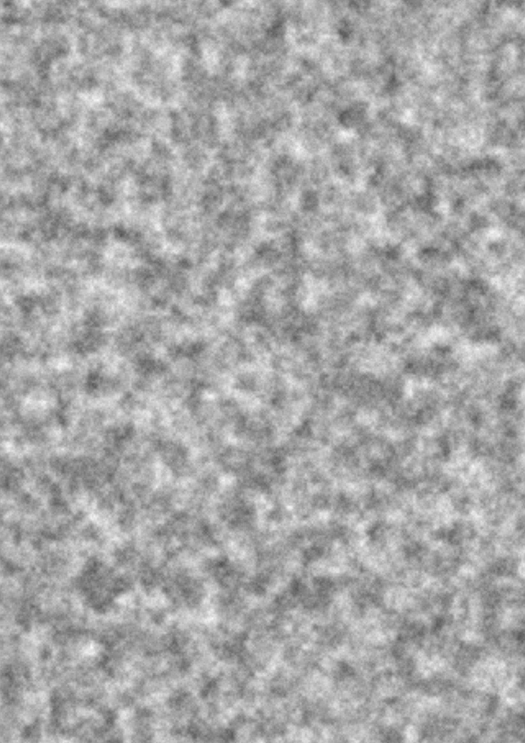
\includegraphics[width=\paperwidth]{title-bg.png}
        };
        \filldraw [fill = white, opacity = .8, thick] ([xshift = .2\paperwidth, yshift = -.25\paperheight]current page.north west) rectangle ([xshift = -.2\paperwidth, yshift = -.5\paperheight]current page.north east);
        \node at ([xshift = .5\paperwidth, yshift = -.375\paperheight]current page.north west) {\Huge\bfseries \parbox[c]{10em}{\centering 高等实分析引论\\ \bigskip\sffamily\large Gerald B. Folland~~著}};
    \end{tikzpicture}
\end{titlepage}

\chapter*{前言}
``实分析''一词首先是指实单变量或多变量函数的经典理论: 极限, 连续性, 微分, Riemann 积分, 无穷级数等相关主题. 然而, 时至今日, 其包含了一些更抽象的理论, 这些理论将实变函数论的思想扩展到更普遍的情形, 又为某些具体的``经典''问题带来了新的启示. 此更高等者乃本书之主题.

故本书的受众为已通晓经典实变函数论者. (关于这些主题有很多书, 古老的经典是\cite{rudin1976principles}, 近来最引人入胜者为\cite{korner2004companion}. 此外, 亦有 Steven Krantz 所著之\,《\,MAA\,导论\,》\,\cite{krantz2014guide}与本书同时问世). 据 MAA 导论之理念, 我将以简明之文对该主题加以阐释, 使入门者览其概述, 研习者深其洞见. 基本定义, 主要定理和证明的关键思想都含于其中, 而不含技术细节. 因此, 书中多数正式陈述结果皆有证明思路随后, 其完整程度差异甚大. 很少或没有提供证明的结果分为两类, 命其``命题''或``定理''以区分之. ``命题''之证明较为简易, 宜供读者以为练习. 若称其为定理, 则意味着其证明较为繁冗且不易删减.

自然, 只有在读者有资源来填补空缺时, 这种介绍方能具有效果. 我把我自己的书\cite{folland1999real}作为内容远比本书丰富的标准参考, 只因为我对它最熟悉. 本书所示均已在\cite{folland1999real}证明, 除了某些明确指明其他来源的结果. 再者, \cite{lang2012real}, \cite{royden1988real}和\cite{rudin1987realcomplex}亦涵盖大部分相同材料.

然而, 本书并非\cite{folland1999real}的简写. 教科书作者的一个主要问题是办法若干相互联系的材料线性叙出, 如同小说家或历史学家一般, 且解决方案并非唯一. 我利用MAA导论所提供的机会, 以一种与\cite{folland1999real}中完全不同的方式来安排这些主题. 读者或可比较二者得见一二.

\begin{flushright}
    {\fontspec{lmromancaps10-regular.otf}Gerald B. Folland}\par\kaishu 西雅图, 二〇〇九年四月
\end{flushright}
\chapter{引论: 记号, 术语和集合论}
\begin{quote}
    在此, 我们简明地讨论一些记号, 术语和集合论的基本事实, 这些结果将贯穿全书.
\end{quote}
\section{数}
命
\[
    \begin{aligned}
         & \mathbb N  =\textit{正整数集},
         & \mathbb Z  =\textit{整数集},   \\
         & \mathbb R  =\textit{实数集},
         & \mathbb C  =\textit{复数集}.   \\
    \end{aligned}
\]
用``两个无穷'', $\infty$(或用 $+\infty$ 以示强调) 和 $-\infty$ 延拓实数系乃人之常情. 在广义实数系 $\mathbb R\cap\{\pm\infty\}=[\,-\infty,\infty\,]$ 中, 任意集合 $E$ 均匀最小上界(上确界)和最大下界(下确界), 用 $\sup E$, $\inf E$ 以记之. 再者, 非负数的无穷求和可在 $[\,0,\infty\,]$ 中良定, 亦即部分和之上确界.

若令 $z=x+\mathrm iy$ 为复数, 其共轭 $x-\mathrm iy$ 用 $\bar z$ 记之, 其绝对值或模 $\sqrt{z\bar z} = \sqrt{x^2 + y^2}$ 记为 $|z|$.

实(复) $n$ 元有序对空间用 $\mathbb R^n$ 或 $\mathbb C^n$表示, 令 $u=(u_1,\dots,u_n)$ 含于 $\mathbb R^n$ 或 $\mathbb C^n$, 则其 Euclidean 范数记为 $|u|$:
\[
    |u| = \biggl( \sum_{j=1}^n |u_j|^2 \biggr) ^{1 /2}
    .\]
自然地, 定义 $\mathbb R^n$ 元素的乘积为
\[
    u\cdot v=\sum_{j=1}^n u_j v_j
    .\]
\section{集合与映射}
现应用集合论的标准记号: $E=F$ 的情形亦可以被 $E\subset F$ 解释, 令其相对补集 $E\setminus F$ 为
\[
    E\setminus F = \{\, x\in E \mid x\in F \,\}.
\]
以 $\varnothing$ 表空集. 不交集族即满足 $\alpha \neq \beta \implies E_\alpha\cap E_ \beta =\varnothing$ 的 $\{E_\alpha\}_{\alpha\in A}$.

若考虑固定底空间 $X$ 之子集, 可简化其补集描述, 记之为
\[
    E^\complement  = X\setminus E.
\]
此时应用 De Morgan 律, 若 $\{E_\alpha\}_{\alpha\in A}$ 是 $X$ 的一组子集, 则
\[
    \biggl(\, \bigcup_{\alpha\in A}E_\alpha \biggr)^\complement = \bigcap_{\alpha\in A}E_\alpha^\complement,\quad\biggl(\, \bigcap_{\alpha\in A}E_\alpha \biggr)^\complement = \bigcup_{\alpha\in A}E_\alpha^\complement.
\]
以 $\mathcal P(X)$ 记 $X$(含 $X$ 和 $\varnothing$) 的全体子集.

令 $X$, $Y$ 为非空集. 以严谨集合论之论述, $X$ 至 $Y$ 的映射乃有序对 $(x,y)$ 的全体 $f$, 其满足 $x\in X$, $y\in X$ 且任意 $x\in X$ 存在唯一 $y\in Y$(以 $f(x)$ 记之)使 $(x,y)\in f$. (自然, 在较为随意的场合可认为映射乃将 $x\in X$ 射往 $f(x)\in Y$ 的``规则''.) 称映射 $f:X\to Y$ 为单射仅当 $x_1=x_2$ 时 $f(x_1)=f(x_2)$; 称其满射若 $\{\,f(x)\mid x\in X\,\}=Y$; 称其双射若单满兼得. 如欲描述匿名映射仅以记号 $x\mapsto y$ 标示 $y$ 是 $x$ 在该映射下之像; 兹举一例: $\mathbb R^2$ 上的平方函数 $x\mapsto x^2$.

每个映射 $f:X\to Y$ 可诱导一个 $\mathcal P(X)$ 至 $\mathcal P(Y)$ 的映射, 仍以 $f$ 记之:
\[f(E)=\{\,f(x)\mid x\in E\,\}.\]
$\mathcal P(X)$ 至 $\mathcal P(Y)$ 的映射 $f^{-1} $ 同理:
\[f^{-1} (E) = \{\,x\mid f(x)\in E\,\}.\]
原像映射 $f^{-1} $ 保持交并补的事实非同小可:
\begin{gather*}
    f^{-1} \biggl(\, \bigcup_{\alpha\in A}E_\alpha \biggr)  = \bigcup_{\alpha\in A}f^{-1} (E_\alpha),\quad
    f^{-1} \biggl(\, \bigcap_{\alpha\in A}E_\alpha \biggr)  = \bigcap_{\alpha\in A}f^{-1} (E_\alpha), \\
    f^{-1} (E^\complement)                               = \left( f^{-1} (E) \right)^\complement.
\end{gather*}
(像映射 $f:\mathcal P(X)\to \mathcal P(Y)$ 保持并, 但若 $f$ 非单则不保持交, 非双则不保持补.)

令 $\{X_\alpha\}_{\alpha\in A}$ 为指标集族. 其 Cartesian 积以 $\prod_{\alpha\in A}X_\alpha$ 记之, 其为所有 $f:A\to \bigcup _{\alpha\in A}X_\alpha$ 且 $f(\alpha)\in X_\alpha$ 的映射构成:
\[\prod_{\alpha\in A}X_\alpha =\biggl\{ \,f:A\to \bigcup _{\alpha\in A}X_\alpha\biggm| f(\alpha)\in X_\alpha,\,\forall \alpha\in A\, \biggr\} \]
若 $X=\prod_{\alpha\in A}X_\alpha$, $\alpha\in A$, 则第 $a$ 个坐标映射 $\pi _\alpha:X\to X_\alpha$ 用 $\pi _\alpha(f)=f(\alpha)$ 定义; 常以 $x$, $x_\alpha$ 替以 $f$ 和 $f(\alpha)$, 且称 $x_\alpha$ 为 $x$ 第 $\alpha$ 个坐标.
\section{Zorn 引理}
很多时候, 特别是处理非常普遍的背景时, 我们需要一个定理来断言某些数学对象的存在性, 却无法明确构造之. 通常, 解决这个问题所需的策略来自一些与偏序集相有关的集合论原理. 必要定义陈列如下.

偏序集乃集合 $X$ 赋予二元关系 $\leqslant $ 满足以下所需:
\begin{enumerate}
    \item 若 $x\leqslant y$, $y\leqslant z$, 则 $x\leqslant z$;
    \item 若 $x\leqslant y$, $y\leqslant x$, 则 $x= x$;
    \item 对任意 $x$, $x\leqslant x$.
\end{enumerate}
称偏序集全序若其满足
\begin{enumerate}[resume]
    \item 若 $x$, $y\in X$, 则 $x\leqslant y$ 或 $y\leqslant x$.
\end{enumerate}
偏序集的极大元是令满足 $x\leqslant y$ 仅有 $x$ 本身的元素 $x$.

例如, $\mathbb R$ 在一般序 $\leqslant $ 全序; 对任意集合 $S$, $\mathcal P(S)$ 以嵌入关系 $\subset$ 为偏序. 若令 $X$ 为其真子集全体, 赋予嵌入关系偏序, 其极大元是补集单元的子集. 无限集合的全体有限子集无极大元.

在一般的存在性原理中, 最耳熟能详的当属 Zorn 引理:
\begin{theorem}[Zorn 引理]
    令偏序集 $X$ 满足其任一全序子集 $L$ 都有上界(亦即, $x\in X$ 使得对任意 $y\in L$ 都有 $y\leqslant x$), 则 $X$ 有极大元.
\end{theorem}
Hausdorff 极大原理是另一知名表述: 每个偏序集都有一个极大全序子集. (事实上, $X$ 的极大全序子集的上界是X的极大元. 反之, 对 $X$ 的极大全序子集全体以嵌入为偏序应用 Zorn 定理, 可得到一个极大全序子集.)

另一个存在性原理是选择公理, 其表述为: 若 $\{X_\alpha\}_{\alpha\in A}$ 是非空集族, 则可在 $X_\alpha$ 元素中择一构建集合 $Y$. 注意到 Cartesian 积 $\prod_{\alpha\in A}X_\alpha$ 中元之值域即是此类集合, 故可将选择公理陈述如下:
\begin{theorem}[选择公理]
    非空集族的 Cartesian 积非空.
\end{theorem}
Zorn 引理蕴含选择公理. (考虑从 $A$ 的子集射往 $\bigcup_{\alpha\in A}X_\alpha$ 满足对 $f$ 定义域内的 $\alpha$ 都有 $f(\alpha)\in X_\alpha$ 的 $f$ 组成的函数族 $\mathcal F$, 若 $f\leqslant g$ 则 $\dom(g)\supset\dom(f)$ 且 $g|_{\dom(f)}=f$, 以此赋予偏序.) 亦可由 Zorn 引理证明选择公理, 但其讨论错综复杂. (与此相关的材料可见 Halmos [7].) 以上原理都不能由标准集合论推出.

正如 Zorn 引理, 此类非构造性存在性定理的使用并非毫无争议, 然而, 大多数数学家认为它们完全合法, 同时, 当构造性方法可用时, 它们往往更富有信息.

\chapter{拓扑}
本章所述为点集拓扑学, 亦名一般拓扑学, 乃用以探究极限, 连续性及集合相关几何属性的抽象数学框架.

\section{度量空间}
二十世纪初, 数学突飞猛进发展, 抽象性, 普遍性大为提升. 彼时, 数学家开创一系列理论, 可广纳万象, 以探究极限与连续之思, 而此前, 此思想只止于 Euclidean 空间中子集, 或是一元, 多元实或复函数.

基于此, Euclidean 空间最直接的推广乃度量空间, 其乃一非空集合 $X$ 赋予一函数
\[\rho :X\times X\to [0,\infty).\]
(一个度量)满足以下所需:
\begin{enumerate}
    \item 对任意 $x$, $y\in X$, $\rho (x,y)=\rho (y,x)$ 成立;
    \item (三角不等式) 对任意 $x$, $y$, $z\in X$, $\rho (x,z)\leqslant \rho (x,y)+\rho (y,z)$ 成立;
    \item $\rho (x,y)=0$ 当且仅当 $x=y$.
\end{enumerate}
可认为 $\rho (x,y)$ 是 $x$ 至 $y$ 的距离. 称上为``度量空间 $(X,\rho)$'', 若 $\rho $ 自明, 则可用度量空间 $X$ 称之.

举数例辅之:
\begin{itemize}
    \item $X=\mathbb R^n~\textit{中子集}$; $\rho (x,y) = (\sum_{j=1}^n|x_j-y_j|^2)^{1 /2}$ ($x$ 至 $y$ 的 Euclidean 度量).
    \item $X=\mathbb R^3~\textit{中单位球}$; $\rho (x,y) = \text{$x$ 至 $y$ 的大圆距离}$.
    \item $X=\mathbb R^n~\textit{中光滑曲线}$; $\rho (x,y) = \text{$x$ 至 $y$ 对应曲线长度}$. (即, $X$ 是一一 $C^{(1)}$ 映射 $\phi :(a,b)\to \mathbb R^n$ 之像, 使 $x=\phi (s)$, $y=\phi (t)$, 则 $\rho (x,y)=\int_s^t|\psi '|$.)
\end{itemize}


\bibliographystyle{alpha}
\bibliography{cite}
\end{document}
